\input{latBegin.txt}

\part{Introduction}
\label{introduction}

\chapter{What do we know about OMFs taxonomy}
\label{whatdoweknowaboutomfstaxonomy}

While the relationship between orchids and Orchid Micorrhizal fungi (\textbf{OMF} hereafter) is known since over a century (Bernard N, 1899; M. C. Rayner, 1927; Rasmussen, 2002; Selosse et al. 2011) and the mechanisms of this symbiosis are beginning to be properly understood, the knowledge from a taxonomical standpoint is still in full evolution.

For many years orchids were thought to interact almost entirely with the members of the \emph{Rhizoctonia} complex. It was later discovered not only that orchids have way more interactions with different fungi also from the \emph{Ascomycetes} phylum, but also that \emph{rhizoctonia} is a polyphyletic group, and was disassembled in different taxa, all members of the \emph{Agaricomycetes}, most notably \textbf{\emph{Sebacinales, Ceratobasidiaceae}} and \textbf{\emph{Tulasnellaceae}} (J.D.W. Dearnaley et al. 2012).

There is also evidence of fungi from the \emph{Ascomycota} phylum, especially in the order \emph{Pezizales} (Selosse et al. 2004, Ouanphanivanh 2008, Waterman et al. 2011), but they are the exception rather than the rule.

The most common and known families of OMFs are in the \emph{Basidiomycota} phylum, especially \emph{Inocybaceae}, \emph{Tulasnellaceae}, \emph{Ceratobasidiaceae}, \emph{Russulaceae}, \emph{Sebacinaceae}, \emph{Serendipitaceae} and \emph{Thelephoraceae} (e.g. Roy et al. 2009, Jacquemyn et al. 2010, Duffy et al, 2018, Taylor et al. 2004).

The knowledge is still lacking in many key aspects though, and more research is needed in order to zoom to a more detailed identification of the OMF

\chapter{Distribution and Ecology of OMFs}
\label{distributionandecologyofomfs}

Orchids depend on fungi for the germination of the seeds and in many cases for the nutrients also in adulthood (Leake J.R. 1994; Rasmussen 1995; Rasmussen \& Whigham 1998), so it is safe to assume that OMFs are everywhere orchids are, that is, in all continents except Antartica (Givnish et al. 2016). This is not the whole tale though, as we know that many OMFs can also turn to a soil free-living saprotrophic ecological niche and form mycorrhizal relationship with plants other than orchids (e.g. Selosse et al. 2014), allowing them to spread to a bigger area.

\emph{Tulasnellaceae, Ceratobasidiaceae,} and \emph{Sebacinales}(\emph{Serendipitaceae} and \emph{Sebacinaceae}) are ubiquitous, varying in their contribution to the total amount of OMFs depending on the area and in the level of specialization for the orchids.
Other families, even though less common, still have a presence in most of the world (Jaquemyn et al. 2015).

Both OMFs and orchids vary in their degree of specialization, from a highly specialized to a more generalist approach (McCormick et al. 2004; van der Heijden et al. 2015).

Many parts of the world are dramatically undersampled though (e.g. all the African continent and most of the tropical areas of the planet), so conclusions are often drew from a limited amount of very specific data.

\chapter{Hypothesis}
\label{hypothesis}

The hypothesis tested in the present work is twofold and can be summarized in the following questions

\begin{itemize}
\item \textbf{Do OMFs taxa from different families occour in different habitats}? We know that different families tend to be more common in different areas but the relative importance of the environmental factors, biotical and abiotical, is still in large part unclear.

\item \textbf{Do OMFs belonging to the same family occur in different habitats?} Even if different families occour in different habitats, what's the distribution of each family, and what are the most important factors that may enable us to predict their presence?

\end{itemize}

\chapter{Importance of phylogenetic relationships}
\label{importanceofphylogeneticrelationships}

In order to understand the distribution and ecology of the OMFs we need to get a better insight of their phylogenesis. In general, mycorrhizal associations are the norm in the plant kingdom, and up to 80\% of plant N and P is provided by mycorrhizal fungi (van der Heijden et al. 2015). This symbiotic relationship is one of the oldest and most important in the Plant Kingdom, and shedding light on the phylogenesis of the OMFs can help us understand the evolution of orchids, their distribution and ecology.

\chapter{Selected Variables}
\label{selectedvariables}

-

\chapter{Performed analysis}
\label{performedanalysis}

\section{Phylogenetic analysis}
\label{phylogeneticanalysis}

The phylogenetic analysis were performed on the sequences deposited by the various papers included in the database.
The **primers ** used were mainly ITS1F, ITS4, ITS3 and ITS4OF, all targeting \textbf{regions} between the 18S rRNA subunit and the 28S rRNA subunit, including the Internal Transcribed Spacers (ITS hereafter) 1 and ITS 2. Those primers were usually universal for \emph{Basidiomycota} or in some cases more specific for \emph{Tulasnellaceae} (like ITS4tul).
Sequence \texttt{DQ520100} from \emph{Tremiscus helvelloides} was used as outgroup.

\begin{itemize}
\item Sequences were aligned using the MUSCLE algorithm and manually trimmed to a visually satisfying overlapping

\item Ugene was used as main GUI, v. 37.0

\item The Maximum Parsimony analysis was performed using TNT, v. 1.1

\item The MCMC was performed using MrBayes, v. 3.2.7a

\item Trees were then visually edited with FigTree v. 1.4.4

\item All parameters are available at https:\slash \slash github.com\slash arteteco\slash FunModels\slash blob\slash main\slash script\slash whatScript.md along with the files to reproduce the analysis.

\end{itemize}

\section{Multivariate analysis}
\label{multivariateanalysis}

Multivariate analysis, specifically Principal Component Analysis (PCA hereafter) and Non-metric Multi Dimensional Scaling (NMDS hereafter), were performed to understand both how do the OTUs from different families cluster together (if they do) and what environmental factors are most relevant.

\subsection{Setting the data up}
\label{settingthedataup}

A few steps had to be done in order to prepare the data for the analysis

\begin{enumerate}
\item  Sequences have been clustered into Operative Taxonomic Units (\textbf{OTU} hereafter), by using cd-hit v. 4.8.1. This process yielded 210 OTUs.

\item  The database was then pivoted in a presence-absence matrix

\item  Using the coordinates for each point, environmental values were extracted using \texttt{GDAL}'s \texttt{Sample Raster Values} tool (Using QGIS v. 3.16 as a GUI) and appended to the dataset

\end{enumerate}

Different families were differently rapresnted in the dataset, with \emph{Serendipitaceae} having two OTUs only, and \emph{Tulasnellaceae} 52

\begin{figure}[htbp]
\centering
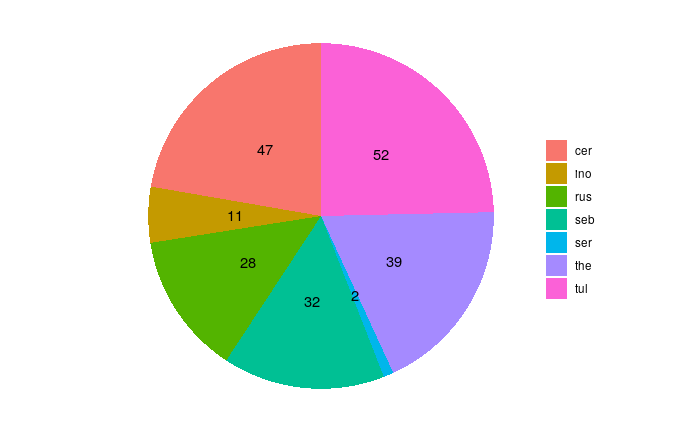
\includegraphics[keepaspectratio,width=\textwidth,height=0.75\textheight]{images/freqFamilies.png}
\caption[title]{Amount of OTUS for each family}
\end{figure}

\section{PCA}
\label{pca}

The PCA was performed on the normalized dataset in two different ways:

\begin{itemize}
\item \textbf{splitting} the families up, so that each matrix only had all the OTUS for a single family;

\item \textbf{lumping} the families up, so that for each family only a single lumping of all the presence\slash absences for those OTUs was used.

\end{itemize}

\section{NMDS}
\label{nmds}

NMDS was simlarly performed on each family's OTUs and on a lumped matrix.

\chapter{Results}
\label{results}

\section{Phylogenetic analysis}
\label{phylogeneticanalysis}

Probably due to the different ways the sequences were originally trimmed and obtained, the phylogenetic results were rather weak.

\begin{itemize}
\item The \textbf{MCMC} had rather low probability branches. Nontheless, it correctly put together the families, with the only notable exception of the \emph{Serendipitaceae} and \emph{Sebacinaceae} which were nested separately. This makes sense though, as they are both \emph{Sebacinales} and the \emph{serendipitaceae} were originally considered \emph{sebacinaceae B} (Weiss et al. 2004) and were only recently given a new name and properly defined (Weiss et al. 2016)

\item The \textbf{Maximum parsimony analysis} was similar, but was not considered to be significative as the Branch Support was in general rather low

\end{itemize}

\input{latEnd.txt}

\end{document}
